
\documentclass{article}
%\usepackage{graphicx}
\usepackage{amsmath}
\usepackage{mwe}
\usepackage{subfig}
\usepackage{float}
\usepackage{xcolor}

\usepackage{graphicx,floatpag,fancyhdr}
\usepackage{lipsum}
\usepackage{hyperref}

% This defines the fancy page style to be similar to plain
\pagestyle{fancy}
\fancyhf{}% Clear header/footer
\fancyfoot[C]{\thepage}
\renewcommand{\headrulewidth}{0pt}% Remove header rule

% Page style plainlower is similar to plain, but lowers page number by 6 lines of text
\fancypagestyle{plainlower}{
\fancyhf{}% Clear header/footer
\fancyfoot[C]{\raisebox{-6\baselineskip}{\thepage}}
\renewcommand{\headrulewidth}{0pt}% Remove header rule
}

%All LaTeX documents have a ``preamble'' that includes the packages and macros needed to make the document compile. The file `PomonaLgcsFormatting.tex' includes the preamble for this template. You can see it in the file list on the left frame of your screen, and this document is instructed to use it with the \input{} command below.


\title{Ny-Alesund O3S-DQA Homogenization Report}
\author{Deniz Poyraz}
\date{\today}

\begin{document}

\maketitle

\section{Ny-Alesund Metadata Timeseries}
\label{sec:metadata}
%Ny-Alesund ozonesonde time series starts in 1992-01. Ozonesonde data were downloaded from the NDACC server and
%DQA homogenization is processed by RMI. Relevant metadata values are extracted from the header of ames data files
%and from the files provided by the station PI. Background (iB2) and pump flow (PF) rate values are missing for 1997.
%For missing values, the median of the relevant value is used.
%The temperature (TLab), humidity (RHLab) and pressure (PLab) values of the laboratory are used for humidity correction.
%When one of these measurements is missing, climatological averages are calculated for each month and these values
%are used for the missing relevant metadata.
%TLab, PLab and ULab are used for pump flow rate moisture correction. iB2 is used for background correction.
%Related plots are shown in \ref{fig:iB2} - \ref{fig:PLab}.
The Ny-Alesund ozonesonde time series was initiated in January 1992.
Ozonesonde data were obtained from the NDACC server and underwent quality checks through DQA homogenization
carried out by RMI. Relevant metadata values were extracted from the headers of Ames data files and
files provided by the station.
The background (iB2) and pump flow (PF) rate values for the year 1997 were not available.
In cases where data was missing, the median value of the relevant data was utilized as a substitute.

For humidity correction, temperature (TLab), humidity (RHLab), and pressure (PLab) values from the laboratory were used.
In instances where any of these measurements were absent, climatological averages were calculated for each month,
and these values were used to fill in the gaps.
Furthermore, TLab, PLab, and ULab were used for moisture correction of pump flow rates, and iB2 was applied for
background correction. Related plots can be found in Figure \ref{fig:iB2} through Figure \ref{fig:PLab}.




\begin{figure}
\centering
\includegraphics[width=0.9\textwidth]{../../Files/ny-aalesund/Plots/Metadata/iB2}
\caption{Ny-Alesund iB2 timeseries}
\label{fig:iB2}
\end{figure}

\begin{figure}
\centering
\includegraphics[width=0.9\textwidth]{../../Files/ny-aalesund/Plots/Metadata/PF}
\caption{Ny-Alesund pump flow rate timeseries}
\label{fig:PF}
\end{figure}



\begin{figure}
\centering
\includegraphics[width=0.9\textwidth]{../../Files/ny-aalesund/Plots/Metadata/TLab}
\caption{Ny-Alesund laboratory temperature timeseries}
\label{fig:TLab}
\end{figure}

\begin{figure}
\centering
\includegraphics[width=0.9\textwidth]{../../Files/ny-aalesund/Plots/Metadata/RHLab}
\caption{Ny-Alesund laboratory humidity timeseries}
\label{fig:ULab}
\end{figure}

\begin{figure}
\centering
\includegraphics[width=0.9\textwidth]{../../Files/ny-aalesund/Plots/Metadata/PLab}
\caption{Ny-Alesund laboratory humidity timeseries}
\label{fig:PLab}
\end{figure}

\section{O3S Corrections}
The code used for processing the homogenization corrections is available at \url{https://github.com/denizpoyraz/o3s-dqa-homogenization}.
\label{sec:v04}


The recommended and applied O3S-DQA corrections are summarized below.
\begin{enumerate}
\item Conversion efficiency
\item Background current
\item Pump temperature measurement
\item Pump flow rate, moistening effect
\item Pump flow efficiency at low pressures
\item Total ozone normalization: in O3S-DQA guide this correction factor is recommended to be added in the data-set,
but the normalization factor is applied.
\item Radiosonde changes: RS80 radiosonde correction is tested but not applied yet.
\end{enumerate}


O3S-DQA corrections are applied to the raw current measured by ECC's. The raw current values are
determined from converting partial ozone values available
in the NDACC files to ECC current for the pre-2017 and are available in ames files starting from 2017
and onwards.

The pump temperature values, pump flow rate and background values (iB2) are needed
to obtain the raw current values.
The corrections applied to calculate ozone partial pressure values in NDACC files, are un-corrected to
get the raw ECC current values. These corrections, applied in the Vaisala software, are:
pressure dependent background correction for SPC sondes and pump flow
efficiency correction.The pump flow efficiency correction table used at this stage is slightly different than
the table used for O3S-DQA pump efficiency corrections.
The correction applied for uncorrecting NDACC pump flow efficiency can be seen in Ozone Sounding with Vaisala
Radiosonde RS41 User's Guide M211486EN, page 74 and the correction table
used for O3S-DQA can be seen in O3S-DQA Activity: Guide Lines for Homogenization of Ozone Sonde Data (Version 2.0)
at page 34.
The Ozone partial values values from the PI station are shown as
'NDACC' and all DQA corrections are denoted by 'DQA'
in the rest of the report.

%
\subsubsection{Conversion efficiency}
No absorption efficiency and stoichiometry correction are needed since 3ml of cathode solution and SPC
$1.0\%-1.0$B probes are used throughout the time series.
%        efficiency correction is applied.
%
%%

\subsubsection{Background current}
The effect of background correction on Ny-Alesund data, using iB2, is shown in Figure~\ref{fig:bkg}.
    If $I_B$ exceeds $I_{B,\text{Mean}}+2\sigma_{IB}$, then $I_B$
    should be replaced by a more representative climatic value $I_{B,\text{Mean}}$, but with a
    larger uncertainty $2\sigma_{IB}$, Figure~\ref{fig:iB2}.


\begin{figure}
\centering
\includegraphics[width=1.3\textwidth]{../../Files/ny-aalesund/DQA_nors80/Binned/Plots/EtaBkg_vs_Eta_alltimerange.png}
\caption{Background current correction}
\label{fig:bkg}
\end{figure}
%%
\subsubsection{Pump temperature measurement}

The truest pump temperature correction is applied according to Eq.13 in the O3S-DQA Guidelines.
Until 1996-12 SPC-5A sondes, and onwards  SPC-6A sondes have been launched.
These periods need different corrections and the effects are shown in Figure~\ref{fig:tpump}.


\begin{figure}
\centering
\includegraphics[width=1.2\textwidth]{../../Files/ny-aalesund/DQA_nors80/Binned/Plots/EtaBkgTpump_vs_EtaBkg_alltimerange.png}
\caption{Pump temperature correction }
\label{fig:tpump}
\end{figure}
%%
\subsubsection{Pump flow rate (moistening effect)}
This correction, Eq.15 of the O3S-DQA Guidelines, is applied and shown in Fig~\ref{fig:pf_ptu}.
Details of the values used for this correction are described in Sec~\ref{sec:metadata}.

%
\begin{figure}
\centering
\includegraphics[width=1.2\textwidth]{../../Files/ny-aalesund/DQA_nors80/Binned/Plots/EtaBkgTpumpPhigr_vs_EtaBkgTpump_alltimerange.png}
\caption{Pump flow rate correction applied}
\label{fig:pf_ptu}
\end{figure}
%%
\subsubsection{Pump flow efficiency}
This correction, Eq.22 of the O3S-DQA Guidelines, is applied using Table 6 of the O3S-DQA Guidelines and
shown in Fig~\ref{fig:pf_eff}.
%The interpolation of the correction factors are made using the pressure. This method gives the same result as doing the interpolation using the logarithm of pressure
%and polynomial fit with an error of less than $0.03\%$.
The effect of this correction is shown in Fig~\ref{fig:pf_eff}.
%
\begin{figure}
\centering
\includegraphics[width=1.2\textwidth]{../../Files/ny-aalesund/DQA_nors80/Binned/Plots/EtaBkgTpumpPhigrPhiEff_vs_EtaBkgTpumpPhigr_alltimerange.png}
\caption{Pump flow rate correction applied}
\label{fig:pf_eff}
\end{figure}
%%

%
The effect of all DQA corrections with respect to no correction (Raw PO3) is shown in Fig~\ref{fig:dqa_all}
and comparison of DQA corrected and
NDACC O3 values is shown in Fig~\ref{fig:fig_dqa_ndacc}.

\begin{figure}
\centering
\includegraphics[width=1.2\textwidth]{../../Files/ny-aalesund/DQA_nors80/Binned/Plots/DQA_vs_Raw_alltimerange.png}
\caption{Effect of all DQA corrections}
\label{fig:dqa_all}
\end{figure}
%
\begin{figure}
\centering
\includegraphics[width=1.2\textwidth]{../../Files/ny-aalesund/DQA_nors80/Binned/Plots/DQA_vs_NDACC_alltimerange.png}
\caption{Comparison of DQA and NDACC O3S values}
\label{fig:fig_dqa_ndacc}
\end{figure}
%%%%
%%%
 \subsubsection{Radiosonde correction}
RS80 radiosonde correction is applied to correct the pressure offset difference.
This correction is not included in the DQA corrections, it is only applied to see its effect.
%It's uncertainity is not implemented in the
%total uncertainity of the ozone partial pressure and also in the final DQA ver.
The effect of RS80 correction is shown in Fig~\ref{fig:rs80}. \\

                        \begin{figure}
        \centering
\includegraphics[width=1.2\textwidth]{../../Files/ny-aalesund/DQA_nors80/Binned/Plots/RS80_vs_noRS80.png}
    \caption{RS80 correction applied}
            \label{fig:rs80}
    \end{figure}
%
%
\section{Comparison plots to AURA MLS v4.0}
The Microwave Limb Sounder (MLS), is one of the four instruments on the Earth Observing System (EOS) Aura satellite.
MLS has been measuring vertical profiles of atmospheric trace gases (including
ozone), temperature, geopotential height, relative humidity,
cloud ice water content, and cloud ice water path, since its
launch in 2004. Global measurements at two fixed solar
times, noon–night, at around 01:30/13:30 LST (local solar
time) are achieved, with the number of profiles over, for example, ozonesonde sites varying between zero and six daily.
Here, the MLS v4.0 data is screened according
to the v4.0 Level 2 MLS Data Quality document, and have compared the satellite overpass measurements
with coincident ozonesonde profiles at Ny-Aalesund. Because
there are multiple profiles crossing at a fixed time,
the profile closest in distance is used for the validation. Both
the noon and night overpasses have been used, as we did
not find significant differences between them.
The homogenized (DQA) and non-homogenized (NDACC) Ny-Alesund data compared with the MLS data are compared
and shown in figures between
\ref{fig:niwav04} and \ref{fig:dqav04_rs80}.

\begin{figure}
\centering
\includegraphics[width=1.2\textwidth]{../../Files/ny-aalesund/MLS/Plots/NDACC_vs_MLS_v04.png}
\caption{ NDACC Ny-Alesund O3S vs AURA MLS v4.0  }
\label{fig:niwav04}
\end{figure}


\begin{figure}
\centering
\includegraphics[width=1.2\textwidth]{../../Files/ny-aalesund/MLS/Plots/DQA_vs_MLS_v04.png}
\caption{DQA Ny-Alesund O3S vs AURA MLS v4.0 }
\label{fig:dqav04_rs80}
\end{figure}

        \section{Total Ozone and Total Ozone Normalization Factors}

Total Ozone Normalization (TON) factors have been calculated with and without DQA corrections. TON factors are
extracted
from taking the ratio of TO values from sonde to the TO values given by satellites. TO from the sonde is integrated until
burst pressure (max. 10hPa) and the residuals, calculated from climatological means, are added.
The corresponding plots are shown in Fig.\ref{fig:ton1} and  Fig.\ref{fig:ton2}.

                                \begin{figure}
        \centering
\includegraphics[width=1.2\textwidth]{../../Files/ny-aalesund/Plots/TON/TON_sonde_nors80.png}
    \caption{TO values calculated with NDACC and DQA corrected ozonesonde data}
            \label{fig:ton1}
    \end{figure}

                                 \begin{figure}
        \centering
\includegraphics[width=1.2\textwidth]{../../Files/ny-aalesund/Plots/TON/TON_satellite_one.png}
    \caption{Relative differences of TON values with respect to satellite data calculated with NDACC and DQA corrected ozonesonde data}
            \label{fig:ton2}
    \end{figure}
\section{Total Ozone and Total Ozone Normalization Factors}

Total Ozone Normalization (TON) factors have been calculated with and without DQA corrections. TON factors are
extracted
from taking the ratio of TO values from sonde to the TO values given by satellites. TO from the sonde is integrated until
burst pressure (max. 10hPa) and the residuals, calculated from climatological means, are added.
The corresponding plots are shown in Fig.\ref{fig:ton1} and  Fig.\ref{fig:ton2}.


    \section{Temporal evolution of the vertical ozone concentrations}
    We calculate vertically resolved ozone trends from the surface to around 30 km for
2000-2020, characterised by stratospheric ozone depletion and recovery, respectively.
    The implemented statistical model to calculate trends is the Long-term Ozone Trends and Uncertainties
    in the Stratosphere (LOTUS) multiple linear regression (MLR) model. This model
uses an independent linear trend (ILT) method as trend term,
which is based on two different, independent, trends to describe the ozone decrease until 1997 (ODS increase) and
the slow ozone increase since the early 2000s (after the
turnaround in ODS concentrations). Additionally, the
LOTUS regression includes two orthogonal components of
the Quasi-biennial Oscillation (QBO), the 10.7 cm solar radio flux, the El Niño–Southern Oscillation (ENSO),
and the aerosol optical depth (AOD). As time-series of Ny-Aalesund only starts at 1992, only the post trends are considered.
    Using only one linear trend and other predictors will be checked and used extensively for a more detailed report.
    The trends using post linear term is shown in  Fig.\ref{fig:trend1}.

                                    \begin{figure}
        \centering
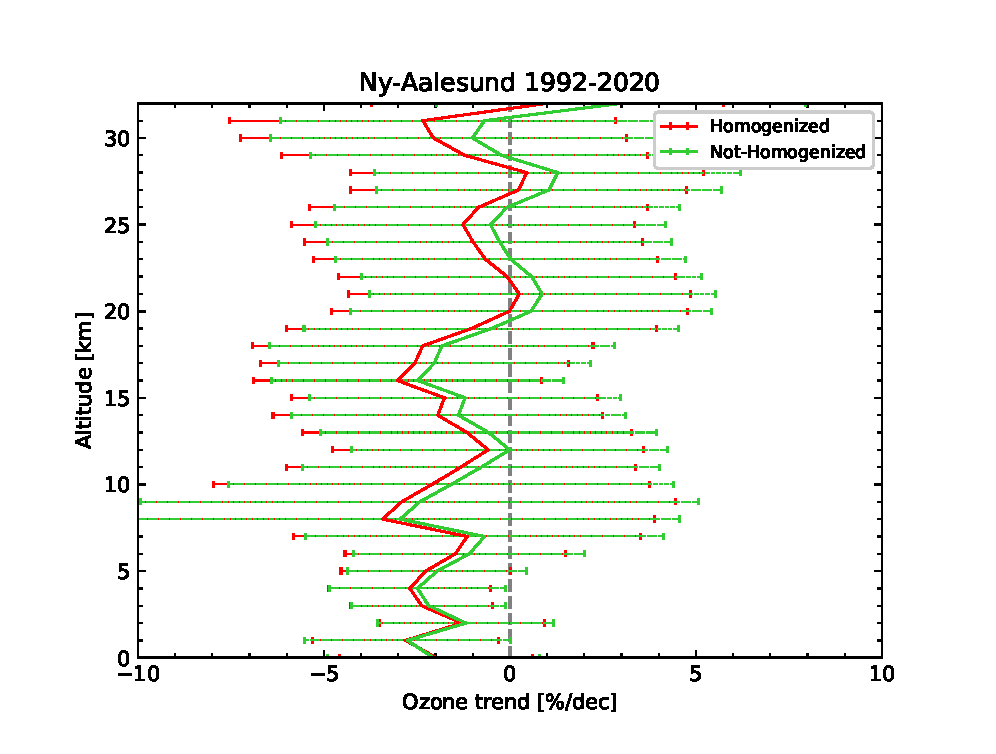
\includegraphics[width=1.2\textwidth]{post_Trend_Ny-aalesund}
    \caption{TO values calculated with NDACC and DQA corrected ozonesonde data}
            \label{fig:trend1}
    \end{figure}

\end{document}
